	\section{Introduction}
	The WorkVisual software package is the engineering environment for KR C4 controlled robotic cells. It offers the following functionalities:

	\begin{itemize}
		\item Configuring and connecting field buses
		\item Programming robots offline
		\item Configuring machine data
		\item Configuring RoboTeams offline
		\item Editing the safety configuration
		\item Transferring projects to the robot controller
		\item Loading projects from the robot controller
		\item Comparing a project with another project and accepting differences where necessary
		\item Managing long texts
		\item Managing option packages
		\item Diagnostic functionality
		\item Online display of system information about the robot controller
		\item Configuring traces, starting recordings, evaluating traces (with the oscilloscope)
		
	\end{itemize}

	\section{Hardware Requirements}
	Minimum requirements
	\begin{itemize}
		\item PC with Pentium IV processor, min. 1500 MHz
		\item 512 MB RAM
		\item DirectX8-compatible graphics card with a resolution of 1024x768 pixels
	\end{itemize}
	Recommended specifications
	\begin{itemize}
		\item PC with Pentium IV processor and 2500 MHz
		\item 1 GB RAM
		\item DirectX8-compatible graphics card with a resolution of 1280x1024 pixels
	\end{itemize}
	
	\section{Software Requirements}
	\begin{itemize}
		\item Windows 7 9Both the 32-bit version and the 64-bit version can be used)
		\item Or: Windows XP (32-bit version, with at least Service Pack 3, the 64-bit version cannot be used)
	\end{itemize}

	If the following software are not already installed on the PC, the installation wizard automatically starts their installation before preceding with the WorkVisual installation.
	\begin{itemize}
		\item .NET Framework 2.0, 3.0 and 3.5
		\item SQL Server Compact 3.5
		\item Visual C++ Runtime Libraries 
		\item WinPcap 
	\end{itemize}
\section{LAN connection}
In order to start file sharing process and to be able to use all functions of WorkVisual, a PC-Controller connection must be established. There are several ways to connect the KRC4 and KUKA-PC, one of which is setting up a local network for the connection of between several devices. This can be done by either setting static IPs for the connected devices and connecting them physically using a specified Ethernet cable, or by using a network router and assign dynamic IPs starting from a specified value, with specified number of connected devices. 
\subsection{To obtain and/or change IP values for the PC}
\begin{enumerate}
	\item Open "Network and sharing center" 
	\item Choose "Change adapter settings"
	\item Right click "Ethernet connections"
	\item  Choose "Internet protocol version 4 (TCP/IPv4)"
	\item  Choose "Properties"
	\item Next you either set static IPs or choose dynamic IPs to be set, in our case by the router.
\end{enumerate}

\begin{mytheo}[address ranges used]
   	The following address ranges are used by default by the
   robot controller for internal purposes. IP addresses from
   this range must not therefore be assigned by the user.
   \begin{itemize}
       \item 192.168.0.0 … 192.168.0.255
       \item 172.16.0.0 … 172.16.255.255
       \item 172.17.0.0 … 172.17.255.255
   \end{itemize}
\end{mytheo}

\subsection{LAN Configuration steps}
\begin{enumerate}
	\item Connect the PC and the KRC4 to the router using regular Ethernet cables.
	\item Access the router configuration page using the given data on the back of the router. (the router used in our case is TP-LINK, with username and password both being \textbf{admin})
	\item In the Interface setup change the LAN settings to your preferred values
	\item It is preferred to set the starting IP address similar to that of the KRC4 (172.31.147) to avoid conflicts. Network gateway value is (172.31.1.1) and subnet mask (255.255.0.0), all other settings shall remain unchanged.
\begin{figure}[h]
  \centering
  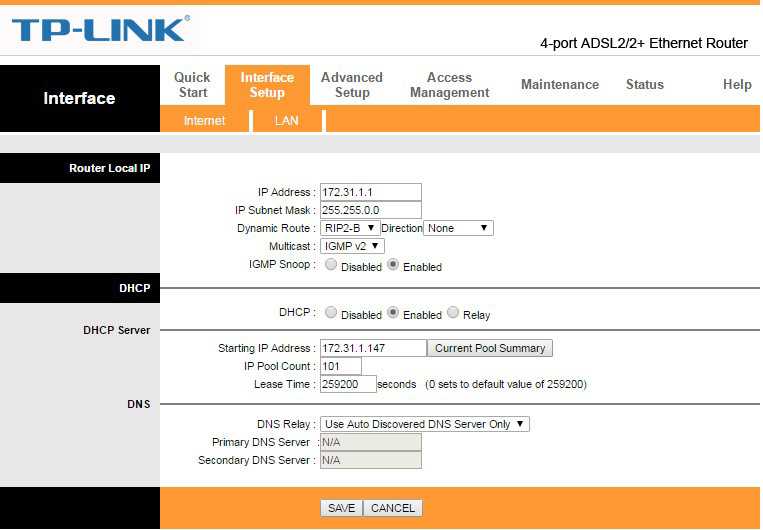
\includegraphics[width=0.9\textwidth]{figures/parts/11}
  \label{fig:11}
  \caption{Router LAN Configuration}
\end{figure}

	\item After changing these values, the IP address used to access the router settings will change from (192.168.1.1) to the set gateway value (172.31.1.1) but with the same user name and password.
\begin{figure}[h]
    \centering
    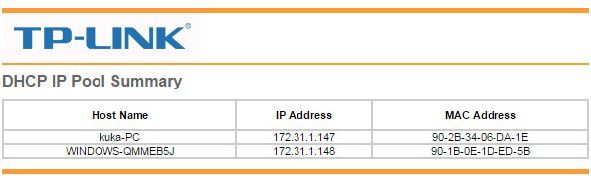
\includegraphics[width=0.9\textwidth]{figures/parts/12}
    \label{fig:12}
    \caption{IP address used to access the router settings }
\end{figure}

	\item The connection is now established and can be verified by checking the router LEDs
\end{enumerate}